
%%%%%%%%%%%%%%%%%%%%%%% file typeinst.tex %%%%%%%%%%%%%%%%%%%%%%%%%
%
% This is the LaTeX source for the instructions to authors using
% the LaTeX document class 'llncs.cls' for contributions to
% the Lecture Notes in Computer Sciences series.
% http://www.springer.com/lncs       Springer Heidelberg 2006/05/04
%
% It may be used as a template for your own input - copy it
% to a new file with a new name and use it as the basis
% for your article.
%
% NB: the document class 'llncs' has its own and detailed documentation, see
% ftp://ftp.springer.de/data/pubftp/pub/tex/latex/llncs/latex2e/llncsdoc.pdf
%
%%%%%%%%%%%%%%%%%%%%%%%%%%%%%%%%%%%%%%%%%%%%%%%%%%%%%%%%%%%%%%%%%%%


\documentclass[runningheads,a4paper]{llncs}

\usepackage{amssymb}
\usepackage{amsmath}
\setcounter{tocdepth}{3}
\usepackage{graphicx}
\usepackage{verbatim}
\usepackage{subcaption}
\captionsetup{compatibility=false}

\usepackage{url}
\urldef{\mails}\path|{willis8, gsherma2, mefron}@illinois.edu|
\newcommand{\keywords}[1]{\par\addvspace\baselineskip
\noindent\keywordname\enspace\ignorespaces#1}

\DeclareMathOperator*{\argmin}{arg\,min}

\begin{document}

\mainmatter  % start of an individual contribution

% first the title is needed
\title{What makes a query temporally sensitive?}

% a short form should be given in case it is too long for the running head
\titlerunning{What makes a query temporally sensitive?}

% the name(s) of the author(s) follow(s) next
%
% NB: Chinese authors should write their first names(s) in front of
% their surnames. This ensures that the names appear correctly in
% the running heads and the author index.
%

\author{Craig Willis \and Garrick Sherman \and Miles Efron}

\authorrunning{}
% (feature abused for this document to repeat the title also on left hand pages)

% the affiliations are given next; don't give your e-mail address
% unless you accept that it will be published
\institute{University of Illinois at Urbana-Champaign \\
501 E. Daniel St., Champaign, IL 61820 \\
\mails}

%
% NB: a more complex sample for affiliations and the mapping to the
% corresponding authors can be found in the file "llncs.dem"
% (search for the string "\mainmatter" where a contribution starts).
% "llncs.dem" accompanies the document class "llncs.cls".
%

\toctitle{Lecture Notes in Computer Science}
\tocauthor{Authors' Instructions}
\maketitle


\begin{abstract}

This work takes an in-depth look at the factors that affect manual classifications of ``temporally sensitive'' information needs. We use qualitative and quantitative techniques to analyze 660 topics from the Text Retrieval Conference (TREC) previously used in the experimental evaluation of temporal retrieval models.  Regression analysis is used to model previous manual classifications. We identify factors and potential problems with previous classifications, proposing principles and guidelines for future work on temporal retrieval models.

\end{abstract}


\section{Introduction}

A basic intuition in temporal information retrieval research is that time should be modeled explicitly when scoring and ranking documents with respect to users' queries. Time-related criteria such as recency, currency, and freshness have long been recognized as factors in studies of relevance \cite{Barry1998}. Based on these criteria, researchers have explored a variety of temporal retrieval models that explicitly incorporate time into the document ranking \cite{Li2003,Efron2011,Dakka2012}. Researchers often refer to general classes of ``temporal queries'' or ``temporal information needs.''  Models have been proposed and evaluated for ``recency queries'' \cite{Li2003,Efron2011}, ``time-sensitive queries'' \cite{Dakka2012}, ``implicitly temporal queries'' \cite{Metzler2009}, and ``temporally biased queries'' \cite{Jones2007}.  For evaluation,  these studies rely on the manual classifications of topics into temporal categories.

In this paper, we take a deeper look into these manually classified topics to develop a clearer understanding of \emph{what makes a query temporally sensitive}?  Previous manual classifications combine the temporal distribution of judged-relevant documents with common-sense notions of topic temporality without a clear explanation of the criteria or processes used in classification. As such, using these manually classified topics for evaluation is of limited value, since the processes being modeled are unclear. 

To address this question, we analyze  660 topics from the Text Retrieval Conference (TREC) previously used in the experimental evaluation of temporal retrieval models. We employ qualitative and quantitative techniques to identify characteristics of topics that might affect the manual assessment of ``temporal-sensitivity.'' The resulting coded topics are used in a set of regression analyses to determine the specific relationships between these characteristics and manually assigned categories. 

This paper is structured as follows: Section 2 presents background information for this study. Section 3 describes the qualitative coding and analysis methods followed by the results in Section 4. Section 5 includes a discussion of the results and conclusions.

\section{Background}

This section presents background information about TREC topics and how they have been classified and used in the evaluation of temporal retrieval models.

\subsection{TREC topics}

Test collections developed for TREC generally consist of a collection of documents, a set of topics and associated relevance judgments. Document collections may be from a single source (e.g., microblog) or composed of multiple sub-collections with distinct start and end dates (e.g., TREC8).  Although the methods of creation have changed over time, TREC topics are generally intended to mimic real users' information needs with respect to the underlying document collection. Topics are distributed in a set of structured text files and typically consist of a title and description.  Temporal information retrieval researchers generally use the topic title as a short query and the title/description for manual analysis and classification.

\subsection{Time and relevance}

There are numerous notions of temporality in information retrieval research, each of which requires different methodologies for analysis. In this study, we are primarily concerned with what we term as \emph{temporal relevance}. We define this as the condition in which information needs are satisfied by documents published at particular points in time. We distinguish this from \emph{temporal topicality} which refers to information needs that are satisfied by documents about certain periods in time. Of course, an information need may combine the two conditions. Examples of studies concerned with temporal topicality include \cite{Berberich2010,Kanhabua2011}.

\subsection{Time-sensitive queries}

In this section, we review examples of studies focused on \emph{temporal relevance}.  The list of topics and collections used in each studies are listed in Table \ref{table.topics}. 

\begin{table*}
\resizebox{\textwidth}{!}{%
\begin{tabular}{| p{2cm} | p{6cm}  | p{6cm} |} \hline
\bf{Topics} & \bf{Collections} & \bf{Studies}\\ \hline
51-200 & TREC Disks 1-2 AP (1988-89) & Jones \& Diaz (2007) \\ \hline
301-450 &  TREC Disks 4-5 FT (1991-94) \newline LA Times (1988-89) & Efron \& Golovchinsky (2011); \newline  Dakka, Gravano \& Ipeirotis (2012) \\ \hline
N1-100 & AQUAINT Xinhua (1996-2000)\newline NYT (1999-2000) & Jones \& Diaz (2007) \\ \hline
851-1050 & Blog06  (Dec 6, 2005 - Feb 21, 2006) & Peetz, Meij \& de Rijke (2013) \\ \hline
MB1-110 & Tweets 2011 (Jan 24, 2011 - Feb 8th, 2011) & Efron, Lin, de Vries (2014)\\ \hline
\end{tabular}}
\caption{TREC topics and collections used in temporal retrieval studies}
\label{table.topics}
\end{table*}

Li and Croft's study of ``recency queries''  \cite{Li2003} was the first to address temporal relevance. They hypothesize that some queries are ``recency queries'' where the most recently published documents are more likely to be relevant.  Through the direct analysis of the temporal distribution of judged relevant documents, they classify 36 of the queries as recency queries because they have ``more relevant documents in the recent past.''

Jones and Diaz \cite{Jones2007} study the temporal characteristics of queries with the goal of query classification through the analysis of three TREC news collections and a web search engine log. They define three classes of queries based on the manual analysis of topics: temporally ambiguous (requesting multiple events),  temporally unambiguous (requesting a single event), and atemporal (having no preference). They employ annotators to  manually classify 100 TREC topics based only on the title, description, and narrative. Specific criteria for classification are not given. For the AP and WSJ collections, they find that all of the queries are either atemporal or temporally ambiguous. As a result, they incorporate the 2003 Novelty track topics because they include topics classified as ``event'' or ``opinion,'' which the authors suggest correspond to the ``temporally unambiguous'' and ``atemporal'' categories respectively.

Dakka, Gravano, and Ipeirotis  \cite{Dakka2012} investigate a broader class of queries which they refer to as ``time-sensitive.'' They hypothesize that there are queries for which more relevant documents are found at specific points in time, not just recently. They manually examine the title, description and narrative of each topic and identify queries associated with specific news events. Only topics with $>20$ judged-relevant documents are considered. If the topic information is insufficient to make a decision, they analyze the distribution of true-relevant documents. The resulting classification consists of 86 temporally sensitive queries. 

Efron and Golovchinsky \cite{Efron2011} investigate additional models for recency queries.  Topics are classified as ``recency'' if at least 2/3 of the relevant documents occur after the median document time and the topic has a ``bona fide temporal dimension'' based on manual review. The specific criteria for manual review are not specified.  

Finally, Peetz, Meij, and de Rijke \cite{Peetz2013a} investigate the effect of temporal bursts in estimating query models. Building on the earlier studies, they evaluate their models using the above test collections as well as a new collection based on TREC Blog06. As in the previous studies, the authors construct a subset of ``temporal'' queries through manual evaluation of topic descriptions and relevant document distributions. No specific criteria for classification are given.

\subsection{What makes a query temporally sensitive?}

We return to the motivating question: what makes a query temporally sensitive? Dakka et al \cite{Dakka2012} present a compelling definition. A query is ``time sensitive''  if  ``the relevant documents for the query are not spread uniformly over time, but rather tend to be concentrated at restricted intervals.''  In other words, a query is temporally sensitive if relevant documents are more likely to occur at some points in time than others. This is an essential point, since many temporal retrieval models rely on the temporal distribution of results in document scoring. However, the distribution of relevant documents alone is not sufficient to determine true temporality. To address this, researchers rely on common-sense notions of temporality based on the topic content considered independent of the distribution of relevant documents. Dakka et al refer to ``newsworthiness''; Efron and Golovchinksy to a ``bona fide temporal dimension''; and Jones and Diaz to ``events.''  A goal of the current study is to look deeper into these common-sense criteria.

In the next section we report the methods used in our analysis of  660 TREC topics used in temporal information retrieval research. 

\section{Methods}

In the studies reviewed above, researchers rely in part on existing TREC test collections to evaluate proposed temporal retrieval models. In each study, topics are manually categorized (e.g.,  temporal or non-temporal) to assess model performance. This study further investigates the characteristics of topics deemed temporal. To achieve this, we use a combination of qualitative content analysis and regression analysis, as described below.

\subsection{Qualitative coding}
We use content analysis \cite{Krippendorff1980} to identify characteristics of TREC topics potentially associated with temporal sensitivity. 660 topics were selected from the TREC Ad-hoc, Novelty, Blog, and Microblog tracks. These topics have previously been used by researchers to evaluate temporal retrieval models. They have associated manual classifications or are from collections with known temporal characteristics (i.e., Microblog). The complete set of topics used in this study are listed in Table \ref{table.topics} along with the temporal constraints of each collection or sub collection.



Two of the authors participated in the development of the codebook and subsequent coding of topics. Codebook development began with a preliminary reading of all topic titles, descriptions and narratives. Codes were defined based on characteristics of topics expected to be related to temporal sensitivity, informed by the literature. Of the 660 topics, 330 were coded by both coders. During this process, code definitions were refined and clarified. In the final coding, only topic title and description were used. The final codebook is presented in Table \ref{table.codebook} in the appendix. Coding was completed using the Dedoose\footnote{http://www.dedoose.com} service.  

\begin{table}
\resizebox{\textwidth}{!}{%
\begin{tabular}{| p{3cm} | p{6cm}  | p{6cm} |} \hline
\bf{Code} & \bf{Description} & \bf{Examples}  \\ \hline
Specific Event & Something significant that happens at a specific time and place. Code title and description in concert, even if title does not contain event specifics. & Mount Pinatubo erruption on June 15, 1991; 2008 State of the Union; Hurricane Hugo \\ \hline
Generic Event & Use this code when the topic refers to more than one specific event or a class or type of event. Only use this code if every instance of the event type would be newsworthy (i.e., a specific event) and the central topic of a news article. & Earthquakes, volcano erruptions, elections, disputes, strikes \\ \hline
Indirect Event Reference & Apply this code to indicate when the topic might be indirectly referring to a *specific* event. Use only if you need to turn to external information to identify potential specific events (e.g., your personal knowledge, wikipedia). Do not use if specific event information is contained in the description. & Legally assisted suicide, related to Kevorkian controversy. Partial birth abortion ban, related to partial birth abortion ban legislation. Surrogacy related to Baby M. \\ \hline
Periodic Event & Apply this code to indicate when an event is periodic, recurring at regular, predictable intervals. Never double-code as SpecificEvent or as an entity even though periodic events are often named entities. & Super bowl, Nobel awards, Oscars, State of the Union \\ \hline
FutureEvent & Apply this code to indicate when a topic refers to a future predicted specific event. Never double-code as SpecificEvent. & 2020 Fifa, 2016 Summer Olympics \\ \hline
Person Entity & Apply this code to identify personal names in topics. & President Bush; Sasha Cohen;  \\ \hline
Place Entity & Apply this code to identify places in topics. Limit to proper names. Also apply to references to nations, governments or government bodies. & Peru; Africa; African; European; Atlanta \\ \hline
Organization Entity & Apply this code to identify organizations in topics. Limit to proper names. Do not apply to references to governments (e.g., United States), use PlaceEntity instead. & Hitachi Data Systems; U.S. Congress; \\ \hline
Other Entity & Apply this code to named entities that are not people, places or organizations. Limit to proper names. Includes movies, books., etc. & Hubble Telescope; The Avengers; Euro	\\ \hline
Explicit Date & Apply this code to identify explicit dates. & 1988; June 15, 1991; October 2007; Monday \\ \hline
\end{tabular}}
\caption{Codebook}
\label{table.codebook}
\end{table}


An example of a coded topic from the 2004 Novelty test collection is presented in Figure \ref{fig.example}.  This topic refers to a specific event and contains place entities as well as an explicit date.  Topic N57 is categorized as an ``event'' by the TREC topic creator and is therefore an unambiguous temporal topic as defined by Jones and Diaz.

\begin{figure}
\begin{equation*}
\small
\begin{split}
\mbox{\bf{Title}:} & \big[(\mbox{East Timor})_{PlaceEntity} \mbox{Independence}\big]_{SpecificEvent} \\
\mbox{\bf{Description}:} & \big[  (\mbox{East Timor})_{PlaceEntity} \mbox{ vote for independence from } \\
	& (\mbox{Indonesia})_{PlaceName} \mbox{ in } (\mbox{August 1999})_{ExplicitDate}\big]_{SpecificEvent}
\end{split}
\end{equation*}
\caption{TREC Novelty 2004 topic N57 example annotation}
\label{fig.example}
\end{figure}

In addition to coding the topics based on the defined codes, the coders assigned a temporal designation to the distribution of relevant documents for each topic. Non-parametric densities were fit to the temporal distribution of relevant documents for topics with more than 20 relevant documents. Each coder reviewed the relevant document distribution along with the total number of relevant documents for each topic and assigned one of four values based on subjective impressions about the degreee of temporal constraint of relevant documents:  too few observations (-1), low or no temporality (0), moderate temporality (1), and high temporality (2). These designations are compared to the ACF and DPS values using Pearson's correlation to determine whether they are useful proxies for the relevant document distribution.
 
After coding all 660 topics, the topic/code matrix was exported for subsequent reliability and regression analysis, as described in the following sections. 

\subsection{Reliability analysis}

For this study, coder agreement is measured using Cohen's $\kappa$ for the classification of the distribution of relevant documents. For the broader qualitative coding task, we use a variation of percent overlap, since coding is performed on arbitrary segments of text. We define the \emph{percent overlap} as:

\[
overlap = \frac{m}{m + u_1 + u_2} 
\]

Where $m$ is the number of excerpts assigned the same code by both coders, $u_1$ is the number of codes assigned to excerpts only by coder 1 and $u_2$ is the number of codes assigned to excerpts only by coder 2. If both coders assign no codes to a topic, this is considered perfect agreement. We report the macro overlap (calculated over all topics), the micro overlap (calculated as a per-topic average).  Per-code overlaps are used to characterize coder agreement within each code.

\subsection{Relevant document distributions}

In each of the four prior studies, the authors acknowledge using the distribution of judged-relevant or pseudo-relevant documents in determining topic temporality. For this study, we use two different measures to represent these distributions: the first-order time series autocorrelation (ACF) and the dominant power spectrum (DPS).

Jones and Diaz \cite{Jones2007} use the ACF created by the temporal distribution of pseudo-relevant documents for a query as a predictor of query temporality. They note that queries with strong inter-day dependencies will have high ACF values, indicating predictability in the time series. The first-order autocorrelation of the time series is defined by Equation \ref{eq.acf}:

\begin{equation}
r_1 = \dfrac{\sum_{i=1}^{N-1} (x_t - \bar{x}_{(1)})(x_{t+1} - \bar{x}_{(2)})}{ \big [ \sum_{i=1}^{N-1}  (x_t - \bar{x}_{(1)})^2 \big ] ^{1/2} \big [\sum_{i=1}^{N-1} (x_{t+1} - \bar{x}_{(2)})^2 \big ]^{1/2}}
\label{eq.acf}
\end{equation}

Similarly, He, Chang, and Lim \cite{He2007} use the DPS as a predictor of the ``burstiness'' of temporal features for event detection. The DPS is the highest power spectrum, estimated using the periodogram. The periodogram is the sequence of the squared magnitude of the Fourier coefficients $\Vert X_k \Vert^2$ indicating the signal power at frequency $k/T$ in the spectrum.  The discrete Fourier transform is defined by Equation \ref{eq.dps}:
\begin{equation}
X_k = \sum_{t=1}^T y_f(t)e^{\frac{2\pi i}{T}(k - 1)t}, t=1,2,....T
\label{eq.dps}
\end{equation}

In this study, both ACF and DPS measures are used to reduce the distribution of judged-relevant or pseudo-relevant documents to a single value for the regression analysis, as described in the next section.

\subsection{Regression analysis}

A primary goal of this study is to determine the characteristics that contribute to the manual judgment of topic temporality. We use logistic regression based on the generalized linear model (GLM) implementation in R. The predictors are binary presence indicators for each of the qualitative codes along with the ACF and DPS of the temporal distribution of true-relevant documents.  The response variables are the binary temporal/non-temporal indicators manually assigned in the four studies.  Model variables are selected using standard step-wise procedures based on the Akaike information criterion (AIC). Coefficients are reported using the log-odds and model fit is assessed using pseudo-$R^2$.

\section{Results}

In this section we report the results of our analysis including a summary of the qualitative codes and their distributions, coder agreement/reliability, and regression models. We also report the results of the comparison of the manual assessment of the distribution of relevant documents as compared to the ACF and DPS values.

\subsection{Codes}

Our qualitative analysis suggests three broad classes: events, named entities, and explicit dates. A basic intuition is that topics focused on specific and important events will have a higher degree of temporal relevance. Following the Topic Detection and Tracking definition, seminal events happen at specific times in specific places, often to individuals or other named entities (e.g., organizations). Perhaps the most essential code is the ``SpecificEvent'' -- something important that happens at a particular time and place. Related to SpecificEvent is the ``PeriodicEvent,'' which refers to an event that recurs periodically, such as the Super Bowl, World Cup, or Olympics. Jones and Diaz \cite{Jones2007} note that many of the early ad-hoc queries were temporally ambiguous, referring to multiple events. We incorporate this concept through the ``GenericEvent'' code, which captures topics concerned with a class of specific events, such as earthquakes, elections, or strikes. While analyzing topics, it became apparent that some topics were likely to be inspired by a specific event, but the event is not referenced in the topic description. This concept is captured through the ``IndirectEventReference'' code. The remaining codes are concerned with the identification of specific types of named entities, which are expected to have some  association with topic temporality, and explicit dates.


\subsection{Code distributions}

Figure \ref{fig.codedist} summarizes the percent of topics in each test collection with each code assigned. From these results, we can see that the Novelty and Microblog  collections have a higher percentage of specific events than the Blog and ad-hoc collections. The ad-hoc collections have a higher number of generic events, which supports the findings of Jones and Diaz \cite{Jones2007}. The Blog, Novelty, and Microblog test collections each have larger numbers of named entities in the topic titles and descriptions.

\begin{figure}
\centering
\begin{subfigure}{.5\textwidth}
  \centering
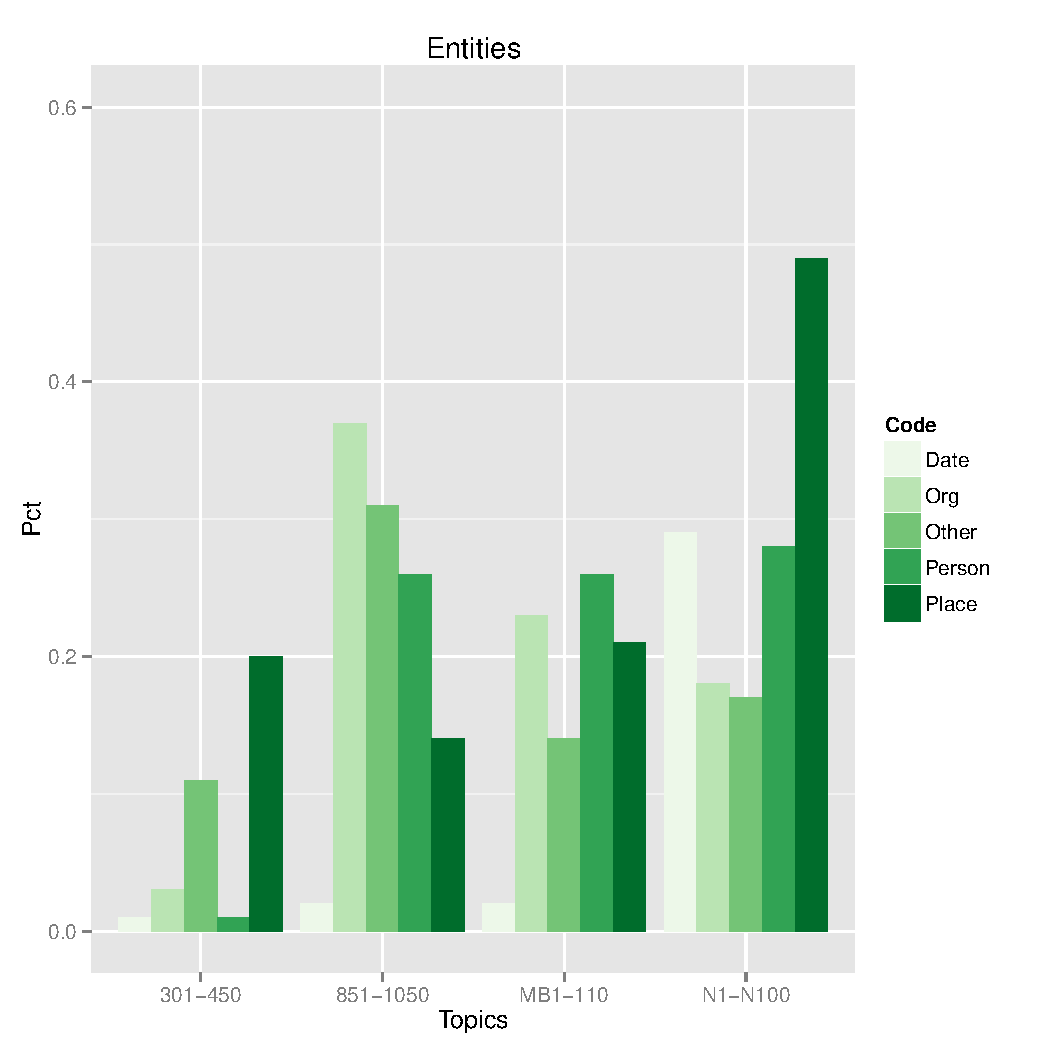
\includegraphics[width=6cm, height=4cm]{plots/topic-groups-ent.pdf}
\end{subfigure}%
\begin{subfigure}{.5\textwidth}
  \centering
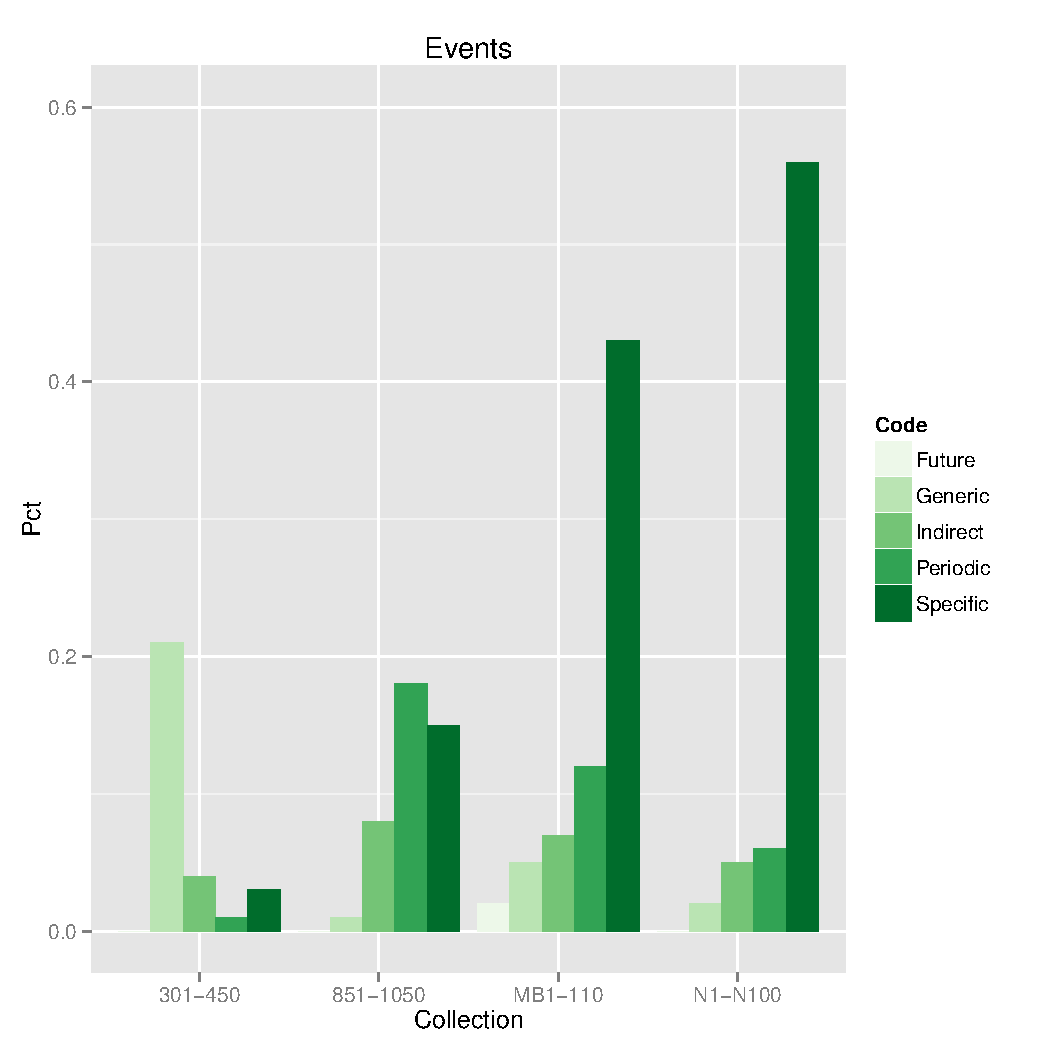
\includegraphics[width=6cm, height=4cm]{plots/topic-groups-evt.pdf}
\end{subfigure}
\begin{subfigure}{\textwidth}
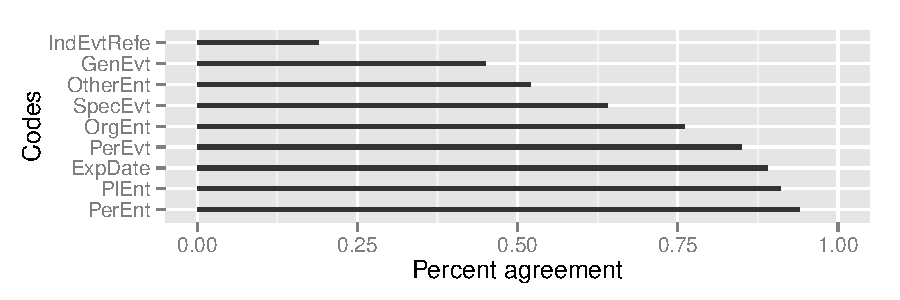
\includegraphics[width=11cm]{plots/coder-agreement.pdf}
\end{subfigure}x
\caption{Percent of topics in each collection with codes assigned from the (a) entity code group and (b) events code group; (c) percent agreement by code.}
\label{fig.codedist}
\end{figure}

\begin{comment}
\begin{table*}
\small
\begin{tabular}{| l | l | l | l | l | l | l | l | l | l | l |} \hline
Topics & ExpDate &	OrgEnt&	OtherEnt&	PersonEnt&	PlaceEnt&	FutureEvt&	GenericEvt&	IndEvtRef &	PerEvt&	SpecEvt \\ \hline
301-450	&	0.01&	0.03&	0.11&	0.01&	0.20&	0.00&	0.21&	0.04&	0.01&	0.03 \\ \hline
851-1050	&	0.02&	0.37&	0.31&	0.26&	0.14&	0.00&	0.01&	0.08&	0.18&	0.15 \\ \hline
N1-N100	&	0.29&	0.18&	0.17&	0.28&	0.49&	0.00&	0.02&	0.05&	0.06&	0.56 \\ \hline
MB1-110	&	0.02&	0.23&	0.14&	0.26&	0.21&	0.02&	0.05&	0.07&	0.12&	0.43 \\ \hline
\end{tabular}
\caption{Percent of topics with each code assigned by topic group}
\label{table.codedist}
\end{table*}
\end{comment}


\subsection{Reliability}

To assess coding reliability, a total of 1244 codes were assigned to 330 topics by the two coders. Higher overlap indicates greater agreement between coders. The macro percent overlap is 0.71 and  micro percent overlap is 0.83, suggesting that overall our codes may be applied with good consistency. The per-code overlap is reported in Figure \ref{fig.codedist}(c). As expected, some codes have higher agreement than others. Specifically, personal names (0.94), locations (0.91), and explicit dates (0.89) have very high agreement whereas indirect event references (0.19) and generic events (0.45) have lower agreement.



\subsection{Regression analysis}

In this section, were report the results of the logistic regression analysis, predicting the manually assigned categories for each test collection. The resulting models are reported in Table \ref{table.regresults}. 

\begin{table*}
\resizebox{\textwidth}{!}{%
\begin{tabular}{| l | l | l | l | l |} \hline
\bf{Name} & \bf{Model}  & \bf{$R^2$} \\ \hline
Novelty 	&  $-3.767 + 5.848 \cdot SpecEvt + 2.523 \cdot Other$& 0.669 \\ \hline
Novelty (Rel)		&  $-3.539 + 7.006  \cdot SpecEvt + 2.530  \cdot Other - 7.343 \cdot ACF$  & 0.706 \\ \hline
Dakka	&  $0.134 + 0.878 \cdot Place$   & 0.019 \\ \hline
Dakka (Rel) 		& $-0.917 + 0.393 \cdot DPS^\blacktriangle$ & 0.263  \\ \hline
Efron	& $-1.765 + 2.353*Place^\blacktriangle + 1.410 \cdot Other^\circ$  & 0.181 \\ \hline
Efron (Rel) 		& $-2.727 + 1.965 \cdot Place^\blacktriangle + 1.787 \cdot Other^\vartriangle + 0.163 \cdot DPS^\blacktriangle$& 0.377 \\ \hline
Peetz & $-0.336 + 1.682*SpecEvt^\circ + 0.982 \cdot PerEvt + 0.672 \cdot Person -0.6175 \cdot Org$ & 0.127 \\ \hline
Peetz (Rel) 		& $-1.245 + 1.218 \cdot SpecEvt + 0.797 \cdot Period + 2.835 \cdot ACF^\circ  + 0.002 \cdot DPS$ & 0.223 \\ \hline
\end{tabular}}
\caption{Logistic regression models for each test collection without and with (Rel) ACF/DPS predictors. Model fit reported based pseudo-$R^2$ after stepwise variable selection based on AIC. Variable significance indicated by $p < 0.05 (^\circ),  < 0.01 (^\vartriangle),  < 0.001 (^\blacktriangle)$ }
\label{table.regresults}
\end{table*}

For the 2003-2004 Novelty collection, the response variable is the manually assigned ``opinion'' (0) or ``event'' (1) categories.  Following Jones and Diaz \cite{Jones2007}, we adopt ``event'' as the temporal category. Logistic regression analysis is performed with and without the ACF and DPS predictors.  SpecificEvent and OtherEntity are significant predictors of the ``event'' category ($p < 0.01$), with a pseudo-$R^2$ of 0.669. Including the ACF of the true-relevant distribution is significant, with a minor improvement in model fit. The high pseudo-$R^2$ is unsurprising in this case, since the SpecificEvent code corresponds to the Novelty ``event'' category. It does, however, confirm our code definition.

Dakka et al manually classified ``time-sensitive queries'' for TREC topics 301-450. As reported in Table \ref{table.regresults}, only the PlaceEntity code is a significant predictor of the manual classification. However, the pseudo-$R^2$ is very low (0.019).  Dakka et al acknowledge examining the relevant document distributions for the Los Angeles Times and Financial Times sub collections.  Including the DPS of the true-relevant document distribution increases the pseudo-$R^2$ to 0.263, suggesting that the relevant document distribution played a significant role in the manual classification.

Efron and Golovchinsky also classified topics 301-450, in this case focusing on the identification of ``recency'' queries. As reported in Table \ref{table.regresults}, both PlaceEntity and OtherEntity are useful predictors of the temporal response. As with Dakka, including the DPS of the true-relevant distribution increases pseudo-$R^2$ from 0.181 to 0.377. This again suggests that the distribution of relevant documents played an important role in the determination of topic temporality.

Finally, we look at Peetz et al's classification of the Blog06-08 topics 850-1050. In this case, the SpecificEvent, PeriodicEvent, Person and Organization entities are useful predictors of the temporal category (pseudo-$R^2$=0.127). Including DPS  improves model fit (pseudo-$R^2$=0.223), again suggesting that the distribution of relevant documents played a role in manual classification.

\subsection{Relevant document distributions}

As described in Section 3.1, non-parametric densities based on the temporal distribution of true-relevant documents are manually classified by two coders into four categories.  The weighted Cohen's $\kappa$ is calculated to assess agreement between the two coders.  Average Pearson's correlation ($\rho$) measures the correlation between these manual classifications and the per-topic ACF/DPS values.  

\begin{table}
\centering
\begin{tabular}{| l | l | l | l | } \hline
\bf{Collection} & \bf{$\kappa$}  & \bf{$\rho_{ACF}$} & \bf{$\rho_{DPS}$} \\ \hline
AP 	   & 0.743 & 0.518 & 0.356 \\ \hline
LA/FT & 0.551 & 0.591 & 0.374 \\ \hline
Blog    & 0.857 & 0.728 & 0.498 \\ \hline
MB      & 0.806 & 0.692 & 0.354 \\ \hline 
\end{tabular}
\caption{Cohen's $\kappa$ for inter-coder agreement for classification of true-relevant document distributions. Pearson's $\rho$ measuring correlation (average) between manual classifications and ACF/DPS values}
\label{table.cor}
\end{table}

The results reported in Table \ref{table.cor} indicate moderate (0.40-0.60) to high (0.60-0.80) agreement between coders and higher correlation between the ACF and the manual classifications. These findings show that ACF and DPS do a good job representing the degree to which relevant documents are temporally constrained. 



\section{Discussion and conclusions}

In this study, we have tried to identify potential factors or characteristics of TREC topics that can be used to predict manual classifications of ``temporal sensitivity.'' Other researchers have classified topics without clear definitions or criteria. We have attempted to model these classifications by proposing features believed to indicate temporality.  Features include the presence of different types of named entities, classes of events, and measures of the temporal distribution of judged relevant documents.

We were successful in modeling the ``event'' and ``opinion'' categories in the TREC Novelty track, based primarily on the presence of our ``SpecificEvent'' code in the analyzed topics.  Event codes were also found to be useful predictors of the classification of Peetz et al. In all cases, the distribution of relevant documents, represented by ACF or DPS, was consistently a significant predictor of topic temporality. 

While these results are promising, we were unable to identify characteristics that fully explain the manual classification decisions. If we cannot explain the process that determines the classifications, it raises questions about the value of these test collections for evaluation. Specifically, how can we be clear that the queries previously identified as ``temporally sensitive'' are truly so? This ambiguity also limits the utility of previous temporal IR research, since it is unclear how to select queries for which temporal models are well-suited.

\begin{figure}
\begin{subfigure}[t]{1in}
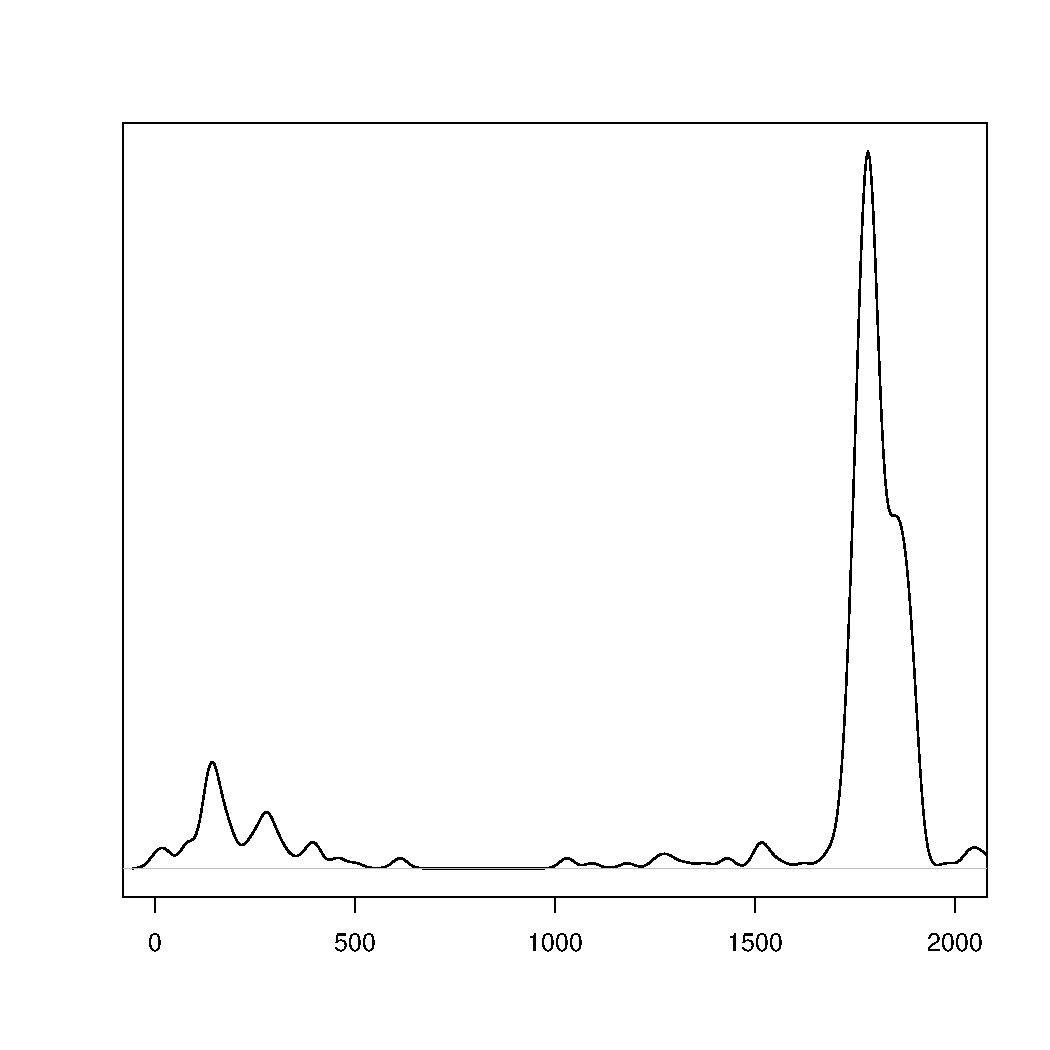
\includegraphics[width=3cm]{analysis/301/301-trec8.pdf}
\caption{All}
\end{subfigure}
\begin{subfigure}[t]{1in}
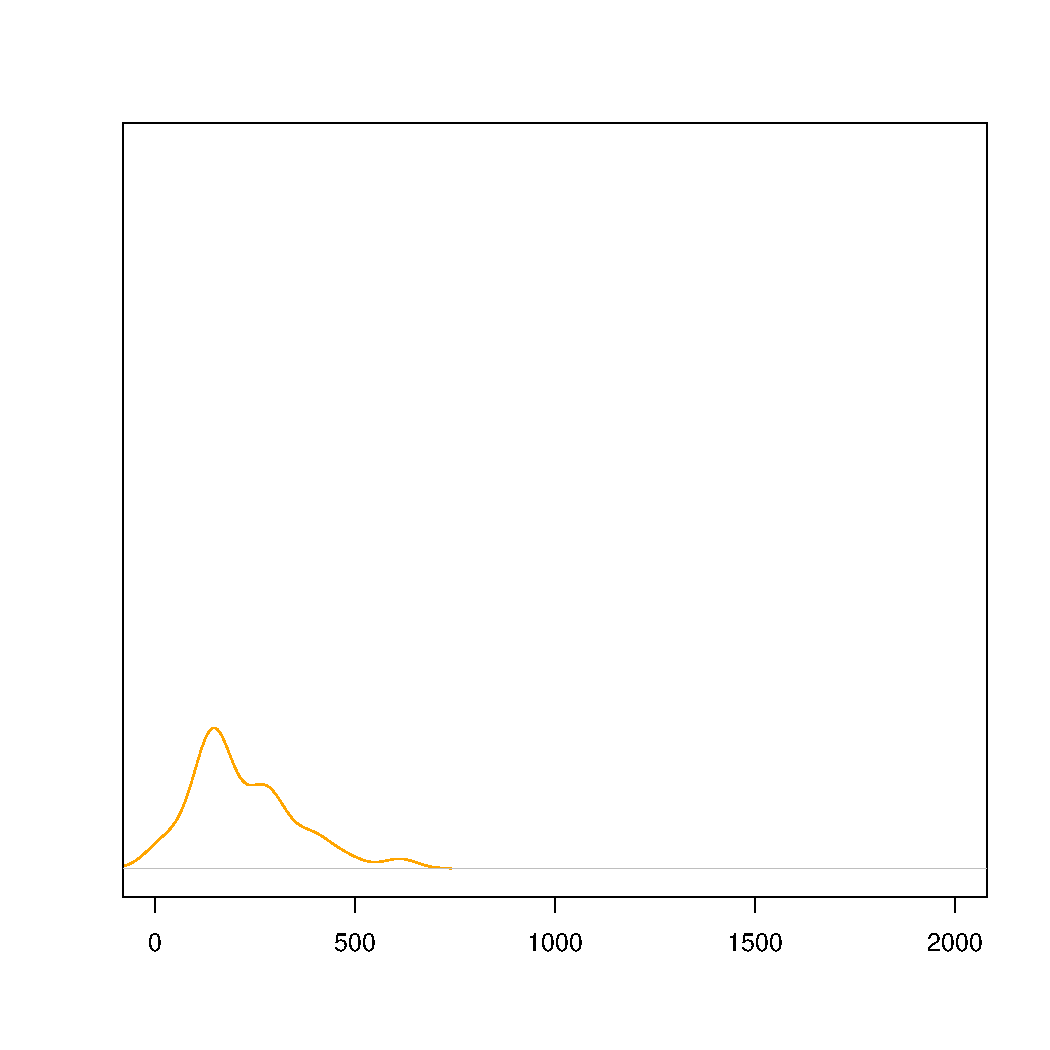
\includegraphics[width=3cm]{analysis/301/301-la.pdf}
\caption{LA Times}
\end{subfigure}
\begin{subfigure}[t]{1in}
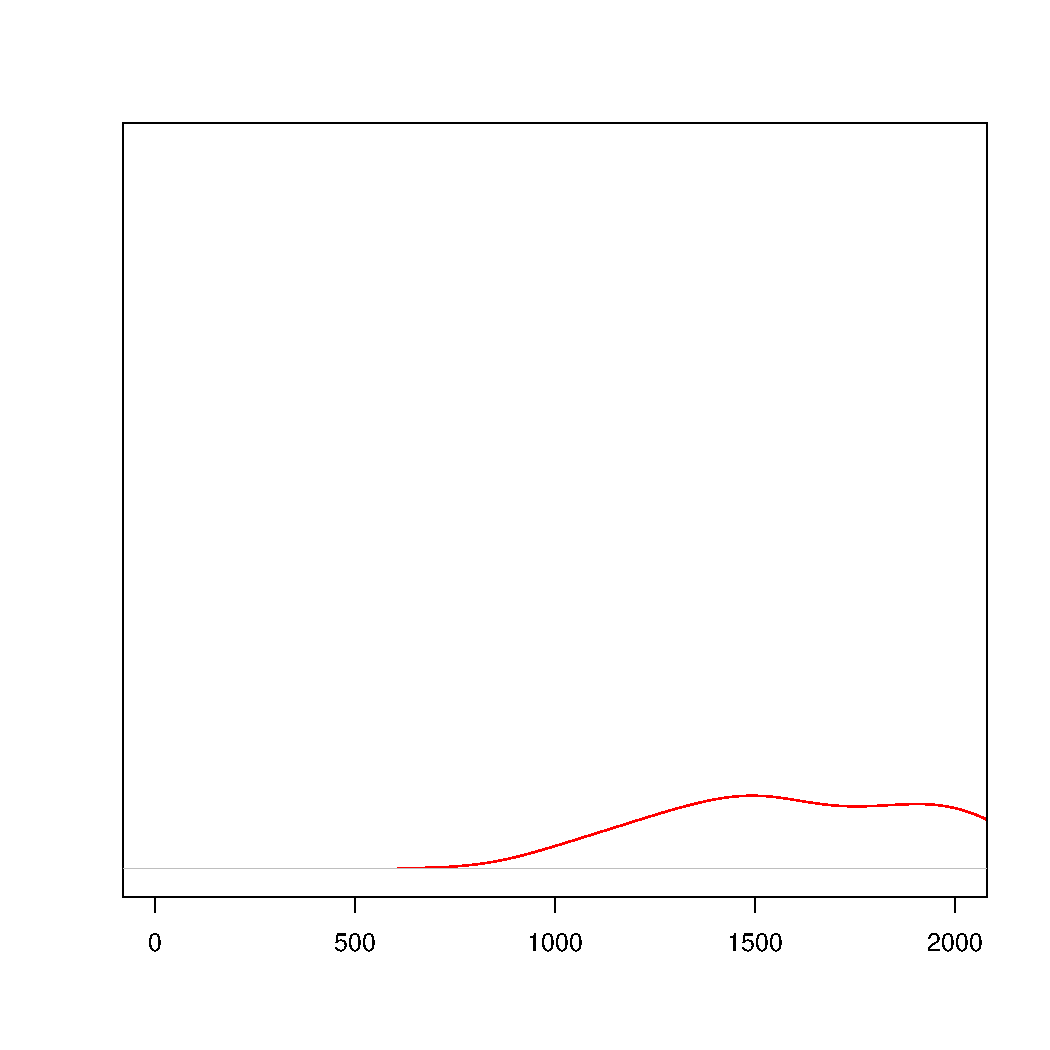
\includegraphics[width=3cm]{analysis/301/301-ft.pdf}
\caption{FT}
\end{subfigure}
\begin{subfigure}[t]{1in}
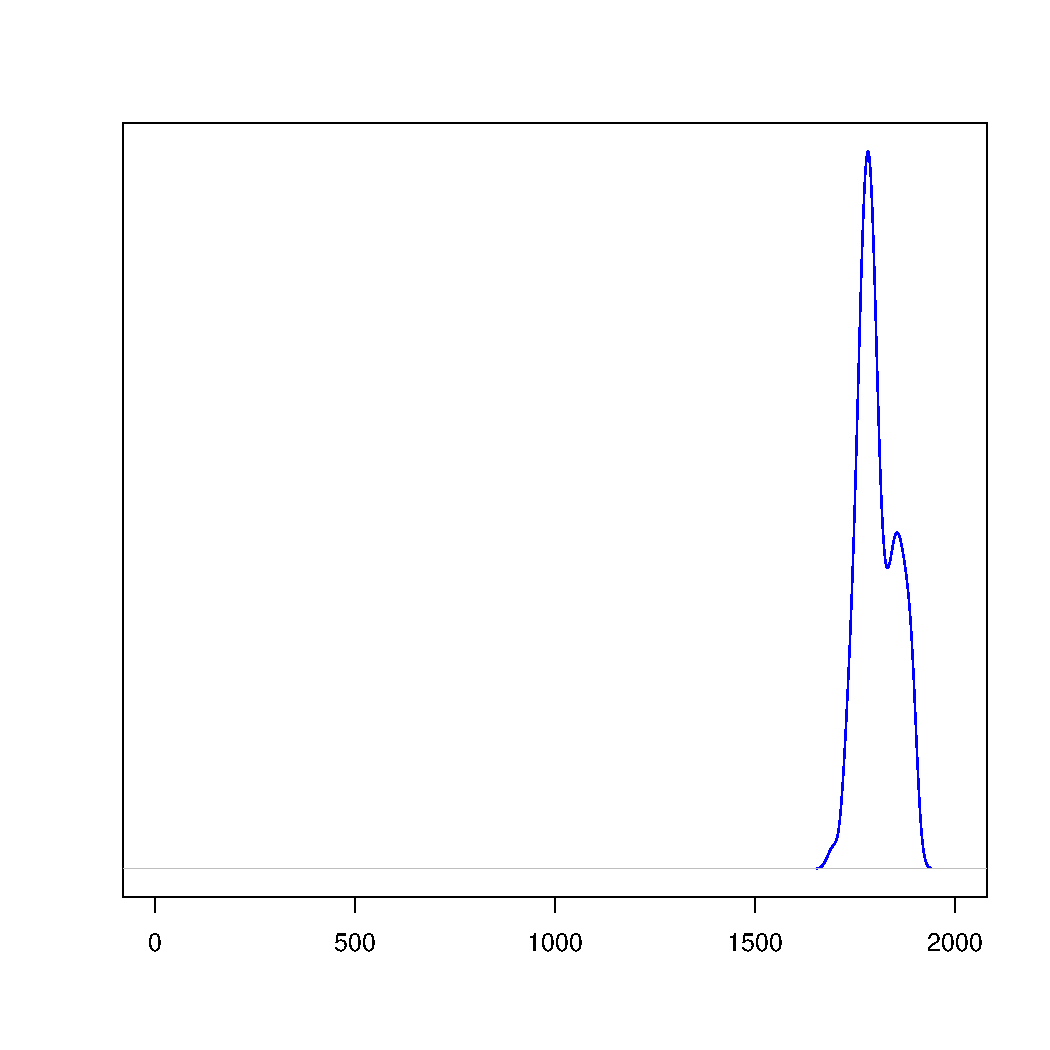
\includegraphics[width=3cm]{analysis/301/301-fbis.pdf}
\caption{FBIS}
\end{subfigure}
\caption{Temporal distribution of relevant documents for topic 301 by sub-collection} 
\label{fig.301}
\end{figure}



We propose a few principles to guide future work on the evaluation of temporal retrieval models.

Aside from the Novelty track topics, the other manual classifications consistently conflate two different concepts: the temporal distribution of judged-relevant documents and a common-sense notion of topic temporality. The temporal distribution of judged-relevant documents is an important indicator of possible temporality, particularly as models often rely on pseudo-relevant document distributions in scoring. However, these distributions alone are not adequate, which is why common-sense criteria have been introduced to determine whether topics have ``bona-fide temporal dimensions.'' We recommend considering these two concepts separately.  Since the first-order autocorrelation of the judged-relevant document distribution is highly correlated with manual judgements of temporality, we recommend using the ACF or other measure of distribution ``burstiness'' or ``peakedness'' instead of manual assessment.  

Common-sense notions of temporality should be clearly explicated.  We found that the presence of different classes of events, as captured in the qualitative codes, would seem to be strong indicators of topic temporality.  This is the case in the Novelty and Blog classifications. As suggested in Figure \ref{fig.codedist}(c), topics 301-450 have fewer specific events, similar to the findings of Jones \& Diaz with the AP and WSJ collections. This suggests that the earlier TREC test collections, including TREC8, may not be well-suited to temporal retrieval research because of the nature of the topics. These collections are also problematic because of different temporal characteristics of individual sub-collections.

Subcollections should be considered independently. Each sub-collection has different temporal dimensions (start/end dates), topical coverage, and document volumes. By combining sub-collections for temporal analysis, researchers risk falsely identifying temporally-sensitive queries. An example is given in Figure \ref{fig.301} which breaks down the distribution of relevant documents by sub-collection in TREC8 for query 301 (international organized crime). This query was used as an exemplar of recency queries in Li \& Croft. Looking at the distribution across all of TREC8, this does appear to be a recency query, since more relevant documents are found toward the end of the collection. However, breaking down the distribution by sub-collection, we see that this is due to a high number of judged relevant documents in FBIS. Though the FT subcollection contains relevant documents during the same time frame as the FBIS spike, the peakedness of that subcollection is significantly less, suggesting considerable differences in the makeup of FT and FBIS. In fact, many of the recency queries in Li \& Croft have large numbers of relevant documents in the FBIS sub-collection.    This leads us to recommend that individual sub-collections should be considered independently.

However, using individual sub-collections is problematic for the LA Times and Financial Times sub-collections, which have surprisingly few judged-relevant documents. The LA Times has an average of 24 and Financial Times 33 judged-relevant documents.  Using Dakka et al's criteria of $>20$ judged-relevant document per topic for the assessment of temporality, only 53 and 70 topics respectively would be available for analysis. This again suggests that the TREC8 sub-collections are not well-suited to temporal retrieval research.
	
\section{Acknowledgments}
This work was supported in part by the US National Science Foundation under Grant Nos. XXX. Any opinions, findings, conclusions, or recommendations expressed are those of the authors and do not necessarily reflect the views of the National Science Foundation. 

\bibliographystyle{abbrv}
\bibliography{temporalir}  

\end{document}
